\chapter{Background}

Malware is a malicious program intended to do pernicious exercises on a client's computer with the proposition of removing data and misusing assets without his assent. Viruses and worms, are best known malwares on account of the way in which they spread, instead of their behavior. Malware is now and then utilized widely against government or corporate websites to gather protected data or to disturb their operations by large. Also, malware is regularly utilized against people to steal data, for example, personal identification numbers or bank or credit card details and passwords. As per a survey on data breaches led by Verizon in 2014, culprits considered Citadel as the preferred banking malware to theft individual information, while Zeus keeps on being the favorite banking malware for stealing money from bank accounts.

Figure 1 shows how the malware is swiftly growing in volume day-byday. In Figure 1, the x-axis specifies the year and the y-axis indicates the number of malware samples generated in the specified year on the x-axis.
\begin{center}
    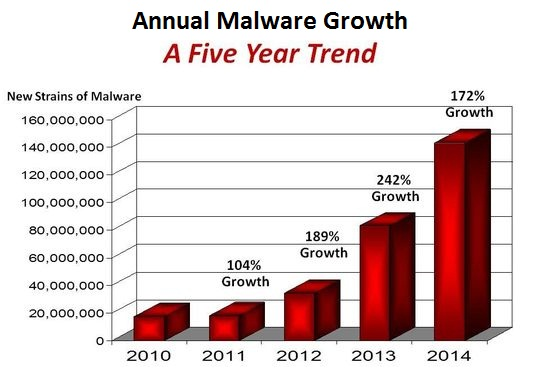
\includegraphics[width=8.4cm, height=6cm]{malware-growth-chart.jpg}
\end{center}
Virus writers are aware, how the signature-based detection with heuristic analysis can be the basis of modern malware detection techniques. So, virus developers have created numerous procedures and techniques to get rid of signature-based detection. In January 2015, AV-TEST's CEO said, "Many of the new malware samples are just variants of existing viruses. They have been modified so that they are no more identified and thus, AV signature updates are required". Some of the noteworthy techniques used by virus writers to evade signature detection are encryption, polymorphism and metamorphism.

\section{Encrypted Malware} 

To typeset text, you type whatever you want. Multiple spaces are
ignored                           when typesetting, and
the end of a line is treated as another space.
Consequently, when you are typing, you can break lines anywhere, like here
or here,
since the lines are formatted automatically when you typeset the document.
You start a new paragraph by leaving a blank line.

See how easy it is to start a new paragraph? A blank line does the trick.

\section{Polymorphic Malware} 

To typeset text, you type whatever you want. Multiple spaces are
ignored                           when typesetting, and
the end of a line is treated as another space.
Consequently, when you are typing, you can break lines anywhere, like here
or here,
since the lines are formatted automatically when you typeset the document.
You start a new paragraph by leaving a blank line.

See how easy it is to start a new paragraph? A blank line does the trick.

\section{Metamorphic Malware} 

To typeset text, you type whatever you want. Multiple spaces are
ignored                           when typesetting, and
the end of a line is treated as another space.
Consequently, when you are typing, you can break lines anywhere, like here
or here,
since the lines are formatted automatically when you typeset the document.
You start a new paragraph by leaving a blank line.

See how easy it is to start a new paragraph? A blank line does the trick.


\section{Transcriptase}

Typesetting text is generally pretty easy. However, there are some special
characters that will not be typeset as you might expect. In the remainder of this
section we consider some of the most common of these
special characters. 

The backslash ``\verb+\+'' is used 
as the ``escape'' character, meaning that
whatever follows a backslash is interpreted as a macro.
For example, when \verb+\LaTeX+ is typeset, it looks like \LaTeX, which 
is a lot different from LaTeX.

To get double quotes, use two single quotes. That is, the left double quote is ``, while the right double
quote is ''. When you do it correctly, quoted text looks ``like this.''
If you use the double quote key, you will always get right-quotes, which looks "like this," and is
almost certainly not what you want.

A tilde ``\verb+~+'' is used as a ``tie,'' that is, a space is inserted, but no line break can occur.
For example, you might type Dr.~Stamp just to be sure that the line of text
does not break between Dr. and Stamp, as it otherwise might.

The percent sign is used for comments---everything following a percent sign 
on a given line is ignored when you \LaTeX\ your file. % Like this stuff here
If you want a percent sign to appear in your document, use \verb+\%+, 
which will give you this \%.

The dollar sign also has special meaning, since it is used to start and end
math formulas. To typeset a dollar sign, use \verb+\$+, like this~\$.

To force \LaTeX\ to insert a space, use a backslash followed by
a space, that is, \verb+\ +. You can put in multiple extra spaces\ \ \ \ \ \ \ if you want.

\section{Rhino}

To change fonts, enclose the text in curly brackets and give the appropriate font command.
For example, to italicize text, {\it do this}, and to get boldface, {\bf this is the ticket}.
Another useful font is {\tt this one}, which produces a typewriter-like font.

